\documentclass{article}

% packages and configurations
\usepackage{hyperref} % reference chapters
\usepackage{algorithm}
\usepackage[toc,page]{appendix} % appendix
\usepackage{animate} % needed for animations and videos
\usepackage{bm} % bold font in equation environments
\usepackage[utf8]{inputenc}	% für Umlaute ect.
\usepackage{fancyhdr} % für header
\usepackage{lastpage} % für footer
\usepackage{extramarks} % für header und footer
\usepackage{amsthm} % math stuff
\usepackage{amsmath} % math stuff
\usepackage{amssymb} % math stuff
\usepackage{color}
\usepackage[procnames]{listings} % code listings
\usepackage{graphicx} % für graphics
\usepackage[toc]{glossaries} % Glossar
\usepackage{color}
\usepackage{tikz}
\usepackage[absolute,overlay]{textpos} %to translate graphics through space
\usepackage{soul}
\usepackage{xcolor}
\usepackage{textpos}
\usepackage{caption}
\usepackage{parcolumns}
\usepackage{enumerate}
\usepackage[ngerman,english]{babel} % Umlaute
\usepackage[T1]{fontenc}    % this is needed for correct output of umlauts in pd
\usepackage[section]{placeins} %forces placeins to stay in section
\usepackage{datetime} % custom dates
\usepackage{afterpage}
\usepackage[section]{placeins}

\definecolor{keywords}{RGB}{255,0,90}
\definecolor{comments}{RGB}{0,0,113}
\definecolor{red}{RGB}{160,0,0}
\definecolor{green}{RGB}{0,150,0}

\lstset{language=Python, 
	basicstyle=\ttfamily\small, 
	keywordstyle=\color{keywords},
	commentstyle=\color{comments},
	stringstyle=\color{red},
	showstringspaces=false,
	identifierstyle=\color{green},
	procnamekeys={def,class}}

\title{Bringing together visual analytics and probabilistic programming languages}
\author{Jonas Aaron Gütter  \\
	Friedrich Schiller Universität Jena  \\
    Matrikelnr 152127 \\
    Prof.Dr. Joachim Giesen \\
    Dipl. Inf. Philipp Lucas
	}

\makeglossaries


\begin{document}


\maketitle

\begin{abstract}
A probabilistic programming language (PPL) provides methods to represent a probabilistic model by using the full power of a general purpose programming language. Thereby it is possible to specify complex models with a comparatively low amount of code. With Uber, Microsoft and DARPA focusing research efforts towards this area, PPLs are likely to play an important role in science and industry in the near future. However, in most cases, models built by PPLs lack appropriate ways to be properly visualized, although visualization is an important first step in detecting errors and assessing the overall fitness of a model. The thesis at hand aim to improve this situation by providing an interface between a popular PPL named PyMC3 and the software Lumen, which provides several visualization methods for statistical models. The thesis shows how arbitrary models built in PyMC3 can be visualized with Lumen using the interface. It becomes clear that even for very simple cases, visualization can contribute an important part in understanding and validating the model, since Bayesian models often behave unexpectedly. Lumen can therefore act as a useful tool for model checking.
\end{abstract}

\pagebreak
\tableofcontents

\newglossaryentry{Bayesian network}
{
  name=Bayesian network,
  description={...}
}

\newglossaryentry{conditional probability distribution}
{
  name=conditional probability distribution,
  description={...}
}

\newglossaryentry{inference algorithm}
{
  name=inference algorithm,
  description={is a key part of a \gls{probabilistic reasoning system}}
}

\newglossaryentry{joint probability distribution}
{
  name=joint probability distribution,
  description={...}
}

\newglossaryentry{marginal distribution}
{
  name=marginal distribution,
  description={...}
}

\newglossaryentry{probabilistic model}
{
  name=probabilistic model,
  description={is a key part of a \gls{probabilistic reasoning system}}
}

\newglossaryentry{probabilistic programming}
{
  name=probabilistic programming,
  description={is something}
}

\newglossaryentry{probabilistic programming language}
{
  name=probabilistic programming language,
  description={is used to create a \gls{probabilistic reasoning system} more effectively than with a conventional programming language}
}

\newglossaryentry{probabilistic reasoning system}
{
  name=probabilistic reasoning system,
  description={consists of a \gls{probabilistic model} and an \gls{inference algorithm}}
}

\newglossaryentry{Turing-complete}
{
  name=Turing-complete,
  description={a turing-complete machine can perform any computation that could theoretically performed by any computer. universally programmable.}
}
\printglossaries
\section{Introduction}
%The overall goal of the thesis is to build an API that makes it possible to a PyMC3 user to get his model visualized in lumen with minimal effort. 
A probabilistic programming language (PPL) provides methods to represent a probabilistic model by using the full power of a general purpose programming language. Thereby it is possible to specify complex models with a comparatively low amount of code. With Uber \cite{bingham2018pyro}, Microsoft \cite{gordon2014probabilistic} and DARPA \cite{Hardesty2015} focusing research efforts towards this area, PPLs are likely to play an important role in science and industry in the near future.
However in most cases, models built by PPLs lack appropriate ways to be properly visualized, although visualization is an important first step in detecting errors and assessing the overall fitness of a model. This could be resolved by the software Lumen which provides several visualization methods for statistical models. Previous to this thesis, PPLs were not yet supported by Lumen. The goal of the master thesis at hand is to change that by implementing an interface between Lumen and PyMC3, a PPL wrapped in a python package, so that exploring PPL models by visual analytics becomes possible. The report starts with explaining the basic concepts of Bayesian statistics, along with the most popular sampling methods used to draw inference from Bayesian models. Following that, the idea of probabilistic programming is introduced, as well as the PyMC3 package as a concrete application and the Lumen software as a means of visualizing the resulting models. Having covered the theoretical aspects, the focus is then laid on practical implementations: The same Bayesian model is built once with and once without PyMC3 and the results are compared, to illustrate the functionality of Bayesian modeling and of PyMC3 in particular. After that the core task of the thesis, the implementation of the interface, is described. For this purpose, operations like model fitting, model marginalization and model conditioning have to be implemented using PyMC3. Also a kernel density estimator is used to generate a probability density function out of samples. Finally, a number of examples are shown to illustrate the usefulness of the visualization, and the thesis is concluded.
\section{Concepts of Bayesian Statistics}
\textit{In this chapter, the theoretical concepts of building statistical models using a Bayesian approach are explained, as well as the methods to draw inference from a model by sampling. The former requires an understanding of basic calculation rules for working with conditional probabilities. These rules are further explained in  \autoref{appendix:Rules of Probabilistic Inference}.}
\subsection{General principle}
\label{subsec: General principle}
Bayesian data analysis can be used for parameter estimation and prediction of new data points. So before doing Bayesian data analysis one has to come up with a model whose parameters can then be estimated by Bayesian methods and that can then be used for prediction. In addition to specifying the model it is necessary to specify prior distributions on the model parameters. This is a major difference to the classical frequentist approach where model parameters are just single points. In Bayesian data analysis model parameters are treated as random variables that follow a probability distribution. So the first step is usually to define these so-called prior distributions. Finding a good prior can be a complex task. A prior should represent the knowledge that the researcher has about the parameter previous to seeing any data.
\paragraph{Parameter estimation}
Once the model as well as the priors are specified, parameter estimation can be performed by applying the Bayes rule to calculate posterior distributions on the parameters, that is, probability distributions on the parameters given the observed data. The Bayes rule allows to invert the order of a conditional probability and goes as follows:
\begin{equation}
p(A|B) = p(B|A) * p(A)/p(B)
\end{equation}
Transferring that to a model with data $X$ and parameters $\theta$, according to \cite{1439840954}, we get:
\begin{equation}
\label{eq:Bayes_formula}
\begin{split}
p(\theta|X) = p(X|\theta) * p(\theta)/p(X)
\end{split}
\end{equation}
Here, $p(\theta|X)$ is the posterior distribution of the parameters. Getting this distribution is equivalent to getting the parameter estimates in the classical frequentist approach. $p(X|\theta)$ is the distribution of the data given the parameters. This is what is specified in the model structure that has to be generated before doing any Bayesian analysis. $p(\theta)$ is the distribution of the parameters without seeing any data. It is the prior distribution of the parameters that has already been set up in the first step. $p(X)$ is the distribution over the data without seeing any parameters. It can be calculated by integrating over the joint distribution of the data and the parameters, but that integral can become difficult to solve with increasing model complexity. However, since the data is known in advance and will not change during the estimation process, it can be treated as a constant and therefore ignored for many applications.

\paragraph{Prediction}
Prediction means giving a statement about how future data might look that was generated by the same mechanism on which the model was learned. To predict new data points it is necessary to get the posterior distribution of the data, that is, the probability distribution over the data variables $x$ given the observed data $X$: $P(x|X)$. New data points can then be generated by sampling from this distribution. It can be calculated by integrating over the joint posterior distribution \cite{1439840954}:
\begin{equation}
P(x|X) = \int P(x,\theta|X) d\theta
\end{equation}
This requires the joint posterior distribution to be known: the probability distribution over the data as well as the parameters given the observed data $p(x,\theta|X)$. The joint posterior can be computed as follows:
\begin{equation}
\begin{aligned}
p(x,\theta|X) &	= p(x|\theta,X) * p(\theta|X) \\
 			& = p(x|\theta) * p(\theta|X)
\end{aligned}
\end{equation}
The simplification in the second step is possible since it is known that $x$ depends solely on $theta$, and not on the observed data $X$. Hence, we can write $p(x|\theta,X) = p(x|\theta)$.

\subsection{Inference through sampling}
\label{subsec:sampling}
As stated in \autoref{eq:Bayes_formula}, using the Bayes formula, we get the posterior distribution the following way:

\begin{equation}
p(\theta|x) = p(x|\theta) * p(\theta) / p(x)
\end{equation}
We get both the likelihood $p(x|\theta)$ and the prior $p(\theta)$ from the model assumptions. The marginalized probability over the data,$p(x)$, however, is more complicated. To compute it analytically we would have to solve the following integral:

\begin{equation}
\begin{split}
p(x) &= \int p(\theta,x) d \theta \\
&=  \int p(x|\theta) * p(\theta) d \theta
\end{split}
\end{equation}
Calculating this integral can be very difficult or impossible since the integral can be multidimensional \cite{1439840954}. So it is not always possible to get the posterior distribution of the parameters analytically. However, there are methods to sample from the posterior distribution of the parameters. These methods are called Markov Chain Monte Carlo methods (MCMC), or Markov chain simulations. A Markov chain is a sequence of events where the probability for each event only depends on the preceding event \cite{Oxforddictionaries}. MCMC methods all have in common that parameter values are drawn repeatedly as some form of such a Markov chain: In each iteration, the parameter values depend only on the values of the preceding iteration. So in each step, values are drawn from a transition distribution $T_t(\theta^t|\theta^{t-1})$. This distribution has to be constructed in a way that it converges to the posterior distribution $p(\theta|X)$. Once it has converged, the parameter draws can be used as samples. Some of the more popular MCMC methods are explained below.
\paragraph{Gibbs Sampling}
Gibbs Sampling assumes that we don't know the joint posterior distribution $p(\theta = \theta_0,...,\theta_n)$, but we do know the conditional distribution $p(\theta_i | \theta_0,...,\theta_{i-1},\theta_{i+1},...,\theta{n} )$ for each quantity $\theta_i$. At first, arbitrary starting points are set for $\theta$, then each $\theta_i$ is drawn from its conditional distribution given the latest values of the other quantities. This is repeated until convergence is achieved
\cite{Martz1994}.
\paragraph{Metropolis}
The metropolis algorithm can be seen as a generalization of the Gibbs sampler \cite{1439840954} and was originally developed to calculate the behavior of interacting molecules without having to compute the multidimensional integrals previously needed for that computation\cite{Metropolis1953}. The algorithm goes as follows : 
\begin{enumerate}
	\item An arbitrary starting location is chosen for each of the molecules. 
	\item For each molecule, a new possible location is proposed. How this new location is calculated is itself a complex task and can be crucial for the performance of the algorithm. For the sake of simplicity we assume here that the proposed location is just randomly chosen in the near vicinity of the old location.
	\item The change of energy in the system introduced by the position change is calculated.
	\item If the proposed location has a lower energy level than the current one, the proposed location is accepted. If it has a higher energy level, it is accepted with
	a probability anti proportional to the energy increase, that is, the higher the energy increase, the lower the chance of accepting the proposed position. After that, the process is repeated up from step 2.
\end{enumerate}
This algorithm is equivalent to sampling from a probability distribution. The molecules represent variables of the probability distribution, their location represents a specific value of the variable and the negative energy of a configuration of molecules represents the probability density of a point in the distribution. The movement of the molecules through space is the Markov chain here. After the algorithm has converged, the distribution of the chosen points resembles the true probability distribution. It is important to note that for this algorithm to work it is necessary that the probability density, apart from a constant factor, can be computed for any given point of the probability distribution since it is needed for evaluating the acceptance of the proposal \cite{1439840954}.

%PYMC3 uses a Metropolis within-Gibbs-sampler (https://docs.pymc.io/developer\_guide.html)
%\paragraph{Metropolis-Hastings}
%\cite{chib1995understanding}
%The Metropolis-Hastings sampler is a generalization of the metropolis sampler where the probability of accepting the proposed point is calculated differently.
%Metropolis Hastings additionally has the ratio between the proposal distributions in it \cite{chib1995understanding}. Metropolis is chosen in a way that these cancel out.
\paragraph{Hamiltonian Monte-Carlo}
The base approach of Hamiltonian Monte Carlo (HMC) is that we have a particle in a multidimensional space where each dimension represents a variable of the target distribution and thus the location $\theta$ of the particle represents a specific point on the target distribution. As in the metropolis algorithm, a starting location is arbitrarily chosen. The difference to the metropolis algorithm now lies in the generation of the new locations. An auxiliary variable $r$ and the parameters $L$ and $\epsilon$ are introduced for this purpose. $r$ represents the momentum of the particle, $L$ is the number of steps to get to one sample, and $\epsilon$ is the step size for one of these steps. For generating one sample point, a change of locations is proposed $L$ times and is accepted or rejected according to the metropolis algorithm. In each of the $L$ steps, $\theta$ and $r$ are updated by using the so-called leapfrog integrator, which is shown in \autoref{eq:leapfrog}. 
%\begin{algorithm}
%	\caption{Leapfrog integrator}
%	\label{alg:leapfrog}
%	$r \leftarrow r + (\epsilon/2)  \, \nabla_\theta \, (log \, p(\theta))$\\
%	$\theta \leftarrow \theta + \epsilon r$\\
%	$r \leftarrow r + (\epsilon/2) \, \nabla_\theta \, (log \, p(\theta))$
%\end{algorithm}
%\\ 
\begin{equation}
\begin{split}
\label{eq:leapfrog}
&r \leftarrow r + (\epsilon/2)  \, \nabla_\theta \, (log \, p(\theta))\\
&\theta \leftarrow \theta + \epsilon r\\
&r \leftarrow r + (\epsilon/2) \, \nabla_\theta \, (log \, p(\theta))
\end{split}
\end{equation}
As one can see, the update process requires gradient information on the log probability density of the target distribution. So this method cannot be applied if gradient information is unavailable. The generated locations here show less random walk behavior and therefore better performance than the algorithms above if the parameters are set properly \cite{hoffman2014no}.

%can reduce complexity from $O(D^2)$ (Metropolis) to $O(D^{(5/4)}$

%auxiliary momentum variable $r_d$ for each model variable $\theta_d$.

%The momentum variables are drawn independently from the standard normal distribution.

%This extended model can be interpreted as a Hamiltonian system, that is,a physical model of particles, where $\theta$ represents a position of a particle in a $d$-dimensional space and $r_d$ represents the momentum of the particle in the $d$th dimension, $p(\theta,r)$.
%If $L$ is too small, the samples will be close to each other. If $L$ is too large, %the steps can loop back and retrace their steps.
\paragraph{NUTS}
The No-U-Turn-Sampler (NUTS) is a self-tuning variant of Hamiltonian Monte Carlo where the number of steps per sample $L$ does not need to be specified at a fixed value anymore. Instead,
it is attempted to stop the process once the maximum distance between initial and proposed point is reached. This maximum is reached when the inner product between $r$ and the distance between initial and proposed point becomes negative. The next iteration would then only decrease the distance  \cite{1439840954}.
%Since this method does not yet guarantee convergence, it is run both forwards and backwards in time, and then stops if it encounters the above mentioned maximum in either direction.
Once the stop is reached, a sample is drawn from all the points that were visited \cite{hoffman2014no}.

%a slice variable $u$ is introduced
%reversibility has to be preserved

%\paragraph{Simple Monte Carlo}
%One of the most basic methods is called Simple Monte Carlo. There we approximate the integral by sampling over the %\begin{equation}
%\int p(x|\theta) * p(\theta) d \theta \approx 1/m * \sum^m p(x|\theta_i),\quad \theta_i \sim p(\theta)
%\end{equation}
%Simple Monte Carlo has a number of disadvantages, so more sophistical methods are generally used, like Gibbs sampling or NUTS.
\subsection{Evaluating models}
%The model can then be validated by predicting new data points and compare this new data to a test data set \cite{1439840954}.


Since a model almost never catches all aspects of reality, it is necessary, after a Bayesian model has been found, to carry out model checks. Traditionally, model checking has been performed by calculating test quantities or test statistics. A test quantity is usually a scalar summary of data and parameters. A test statistic is also a summary of data, but is conditioned on a fixed set of parameters. It can be used in Bayesian as well as in non-Bayesian contexts. Those summaries are then used to compute a tail-area-probability, also called p-value. In the case of a test statistic, the p-value gives the probability that, given a parameter $\theta$, a test statistic $T$ for replicated data $y^{rep}$ is greater or equal the test statistic  for the observed data $y$, as shown in \autoref{eq:classical_p}:
\begin{equation}
p_C = Pr(T(y^{rep}) >= T(y) | \theta)
\label{eq:classical_p}
\end{equation}
\cite{1439840954}\\
The p-value for a test quantity, on the other hand, is not conditional on a fixed $\theta$ since in Bayesian statistics parameters are drawn from a distribution the same way as outcome variables. Instead, the observed data $y$ is the fixed quantity for the Bayesian p-value, as shown in \autoref{eq:bayesian_p}
\begin{equation}
p_B = Pr(T(y^{rep},\theta) >= T(y,\theta) | y)
\label{eq:bayesian_p}
\end{equation}
\cite{1439840954}\\
If a test quantity has a p-value close to 0 or 1, the aspect that is analyzed by the test quantity is not well captured in the model.\\
Gelman \cite{gelman2004exploratory} argues that visualization can be seen as an alternative form of model checking. He even claims that "when more complex models are being used, graphical checks are more necessary than ever to detect areas of model misfit" \cite{gelman2004exploratory}. In graphical model checking, the visualization plays the role of the test quantity. Even though test quantities are usually scalars, one can also compute them as vectors so that they can be displayed graphically \cite{gelman2004exploratory}. I conclude from this that, when we take this one step further, the data and the parameters can be seen as a vector summary of themselves, so by displaying them, as it is done in this thesis later, we are performing a regular model check according to the proceedings described above.

%In Bayesian analysis, both the prior and the likelihood distribution can be sources of error.
%
%Different models can lead to different posterior inferences, even if both models have a good fit.
%
%model checking: How good does the model fit the data?
%Sensitivity analysis: Comparison of different models with good fit
%
%This is necessary after a joint probability density and a posterior density are calculated. How good are the prior and the likelihood model?
%\textit{Sensitivity analysis} deals with the question, how much the posterior is changed when one chooses a different (but also reasonable) model for the likelihood or the prior, or other assumptions affecting the posterior.
%
%In theory: Setting up a 'super-model' as joint-distribution which includes all possible realities. Posterior of this super-model then automatically incorporates the sensitivity analysis. In practice this is conceptually and computationally infeasible and also is still dependent on the assumptions made when creating the super-model being correct.
%
%One way is just to compare model predictions with the actual outcomes (this is referred to as external validation). If for some reason it is not possible to get the actual outcomes (for example if they lie in the future), one needs to approximate external validation with the available data.
%
%\textit{Posterior predictive checking}: Use global summaries of the data distribution and the predictive distribution to evaluate the model: Draw random samples from the predictive distribution, compare e.g. the smallest of these values with the smallest value in the data...
%

%
%Graphical comparison of simulated and data histograms (!! maybe here point out usefulness of Lumen)
%
%
%p-value depends on the chosen test quantity.
%
%
%Bayesian predictive checking: choose and compute test quantities for the data and for simulations, then compute the p-value for the test quantity (probability that the test quantity of the data could have arisen under the model)
%
%Test quantities give information about a specific aspect of the observed/simulated data. A model can predict values that are in some aspects similar to the data, in other aspects different. Therefore it can make sense to compute p-values fur several different test quantities.
%If a test quantity is dependent on the model parameters it has to be simulated both for the observed as well as for the predicted data. This makes it possible to compare both test statistics (for observed and for simulated values) point wise, eg. in a scatter plot or in a histogram of the differences. The scatter plot should be symmetric around the 45 degree line, the histogram should include 0 (and be symmetric around 0??).
%Test quantities are most useful when they measure an aspect that is not directly recognizable in the probability model.
%Graphical visualization can be used to identify useful test quantities.

%\\
%Model checking depends on the data-collection model (how the data was collected), since data has to be replicated for computing a p-value. Posterior Inference however does not depend on the data collection model, as long as the likelihood model stays the same. Because of this, the same posterior results(what are the parameters) can get different model checking results (how well does the model fit) when the data-collection model is changed.
%\\
%Marginal predictive checks: Instead of replicating data from the joint posterior distribution, one can also compute the probability for a certain outcome, and compare this probability with the data....(p.153).
%\\
%Graphical posterior predictive checks: Basic Idea: Visualize the data alongside simulated data and so find discrepancies --> perfect in Lumen 
%Possibilities:
%\begin{itemize}
%	\item Direct display of all the data
%	\item Display of data summaries (e.g. if the data is so large that it is not helpful to display all the data)
%	\item Display a measure of discrepancy between model and data
%\end{itemize}
%
%MAYBE BUILD EXAMPLES WITH LUMEN TO ILLUSTRATE USEFULNESS OF LUMEN
%\paragraph{Direct data display}
%
%Show the complete data and its correspondent simulations. It's best to show several replications.
%
%\paragraph{Display data summaries}
%
%\paragraph{Display discrepancy measures}
%Bayesian residuals are defined by $y_i - g(x,\theta)$, where, in contrast to classical residuals, $\theta$ is not a point estimate of parameters, but a single draw from the posterior distribution of the parameters.
%
%Difficult with discrete data, since residuals can only take certain discrete values. Graphical visualization can then be misleading since the discrete values can suggest patterns. To avoid this, one can use \textit{binned residuals}, that is plotting the averages over a number of residuals and their corresponding outcomes. 

%According to Gelman et al.  \cite{1439840954}, it is also useful to compare summaries of the data (such as the mean) to summaries from posterior simulations. 
%Gelman et al \cite{1439840954} name three kinds of graphical display, that are suited to validate models:
%- Direct display of data
%- Display of data summaries
%- Displaying measures of discrepancy

%This process of comparing observed to simulated data in a Bayesian context is called posterior predictive checking.


% In Lumen: One can check the models behaviour, that is, the interaction of pairs of variables.
% Gelman et al \cite{1439840954} describe drawing data from the posterior distribution and then comparing it to the training data as a means of validating a model. With PyMC3 and Lumen, we can actually do even better and compare the actual posterior distribution to the training data.
% Comparison of summaries is not possible in Lumen since it only shows the actual data, no summaries.

%\subsection{Choosing an appropriate prior distribution}
%\label{Choosing an appropriate prior distribution}
%There are two interpretations of prior distributions. The \textit{population} interpretation, where the prior distribution is thought of as a population of possible parameters, from where the current parameter is drawn. This, as far as I understand, requires the range of possible values to be known, e.g from past experience. On the other hand, the \textit{state of knowledge} interpretation looks at the prior distribution as an expression of the user's knowledge or uncertainty, so that the assumption is plausible, that the real parameter value is taken from a random realization of the prior distribution.
%\\
%When we have lots of knowledge about the parameter already, it makes sense to choose an \textit informative prior, which has a big influence on the posterior distribution.On the other hand, if one does not want prior beliefs to affect the outcome of an analysis, one should not choose informative priors, even when lots of knowledge is available. E.g. when testing a hypothesis, it is not wise to include information in the prior that supports the hypothesis for fairness reasons(?? look that up again on p. 56.). If there is no sufficient data to estimate a prior, it is desirable to choose a prior that is \textit non informative, meaning that it will contribute very little to the posterior distribution ('let the data speak for itself'). A common non informative prior, motivated by Laplace's principle of insufficient reason, is the uniform distribution. However, the uniform distribution is not ideal since it is dependent on the parametrization: Applying a uniform distribution to $p(x)$ leads to a non-uniform distribution when looking at $p(x^2)$ and the other way round \cite{1439840954}. Jeffrey's approach to find noninformative prior distributions negates this problem by choosing a prior that is invariant to the parameterization (see https://eventuallyalmosteverywhere.wordpress.com/2013/05/10/bayesian-inference-and-the-jeffreys-prior/).
%Besides informative and noninformative prior distributions there is also the \textit {weakly informative} prior distribution. This kind of prior does affect the posterior distribution in terms of regularization (e.g. it prevents extreme outliers), but it does not contain any further special knowledge about the parameter. A normal distribution with high variance is often used as weakly informative prior.
%\\
%The parameters of the prior distributions are called hyperparameters. The property that prior and posterior distribution are of the parametric form (e.g., both are a beta distribution) (for a given likelihood distribution), is called conjugacy. Conjugate prior distributions have the advantages of being computationally convenient and being interpretable as additional data.
%\\
%A prior distribution is called \textit{proper} if it does not depend on data and sums to 1 \cite{1439840954}. Proper distributions can be normalized. The uniform prior for example is \textit{improper}, since it can't be normalized.
%
%\subsection{Sampling distribution}
%\label{Sampling distribution}
%
%The sampling distribution, also called the likelihood of the data.
%\\
%Often it is about which distribution class should be chosen for the prior and the likelihood. Standard, convenient distributions for single-parameter models: normal, binomial, Poisson, exponential. Those can also be combined to represent more complex distributions. For different classes of sampling distributions there are corresponding conjugate prior distributions which lead in turn to posterior distributions of the same form. \cite{1439840954}
%\\
%distributions can be chosen for mathematical convenience. One could estimate hyperparameters of the likelihood distribution from the data in some cases. This is a bit of a circular reasoning, but apparently  it is appropriate for \cite{1439840954}.

%\subsection{Stuff that has to be/could be placed somewhere}
%
%
%\subsubsection{Posterior distribution}
%
%The posterior distribution is a compromise between the prior distribution and the sample distribution, with the prior distribution becoming less important as the sample size increases \cite{1439840954}.
%posterior distributions can be described numerically by mean, median, modes. The uncertainty can be described by quantiles. The highest posterior density region is also a possibility, it is the area that for example contains 95\% of the posterior probability density, like quantiles, but has the additional constraint that the density on each point inside the area has to be bigger than the density on any point outside the area. It does not have to be one single connected area  \cite{1439840954}.
%\\
%For the posterior distribution, a normal distribution is often assumed.
%
%\subsubsection{Drawing inference}
%According to \cite{Wang2018}, the likelihood of a new data point can be calculated by integrating the product of the prior likelihood and conditional probability of $\beta$ over the space of $\beta$, as shown in equation \autoref{eq:posterior_predictive}. This formula can also be derived using the chain rule (I think).
%\\
%If it is not possible to perform calculations directly from the posterior distribution (e.g. if there is no closed form but only a discrete approximation of the posterior distribution), one can simulate data points from the posterior distribution instead and perform calculations on them \cite{1439840954}.
%
%\begin{equation}
%p(x_{new}|\boldsymbol x, \alpha) = \int p(x_{new}|\beta) * p(\beta | \boldsymbol x,\alpha) d \beta
%\label{eq:posterior_predictive}
%\end{equation}

\section{Probabilistic Programming Languages}

\textit{In this section, the idea of Probabilistic Programming is explained. It is defined what a Probabilistic Programming Language(PPL) is, and a number of PPLs are introduced. A Bayesian model is created once with and once without a PPL, and the results are compared.}

\subsection{Probabilistic Programming}
According to Pfeffer \cite{9781617292330}, probabilistic programming is the process of creating a probabilistic reasoning system with the means of a programming language. A probabilistic reasoning system is, in turn, a structure that uses knowledge and logic to calculate a probability. Here, knowledge can be interpreted as data about certain quantities, and logic can be interpreted as the knowledge about how these quantities interact and influence each other. Pfeffer \cite{9781617292330} uses the example shown in \autoref{fig:example_prs} to illustrate the functionality of a probabilistic reasoning system. There, we want to calculate the probability of scoring a goal by a corner kick during a game of soccer. The probabilistic reasoning system includes general knowledge about the situation, for example, that overall 9\% of corner kicks result in a goal. That is what is called the korner-kick model in the example. Additional data about the circumstances of this particular situation are given to the system as evidence. In the example, these circumstances are a tall center forward, an inexperienced goalie and strong winds. The system now uses this data, together with its logic of how each circumstance affects the outcome, to calculate probabilities for a given event, here, the scoring of a goal. The part of computing these probabilities is called inference algorithm in the example.
\begin{figure}
	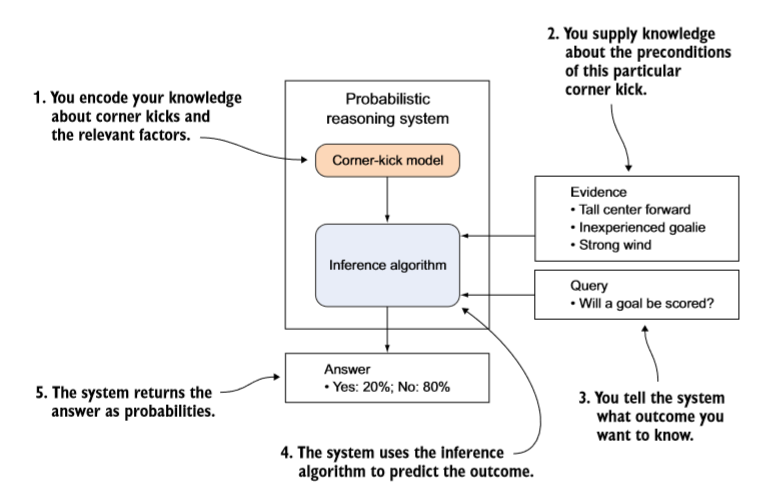
\includegraphics[width=\textwidth]{images/probabilistic_reasoning_system.PNG}
	\caption[General workflow example of a probabilistic reasoning system. Source: \cite{9781617292330}]{General workflow example of a probabilistic reasoning system}
	\label{fig:example_prs}
\end{figure}
From a data science perspective, this means that a Probabilistic Programming Language(PPL) provides ways of describing a probability model and drawing inference from it, which, in the ideal case, are more flexible, more efficient, and better to understand than traditional approaches \cite{Hardesty2015}. Currently, a number of PPLs is publicly available, with the most popular being mentioned below:
\paragraph{Stan}
is an open-source program written in C++ that is designed for Bayesian inference on user-specified models. As described in \cite{Gelman_2015}, it consists of the following components:
\begin{itemize}
	\item A modeling language that allows users to specify custom models
	\item An inference engine which uses Hamilton Monte Carlo methods for sampling to get an approximation for the posterior distribution
	\item An L-BFGS optimizer for finding local optima
	\item Procedures for automatic differentiation which are able to compute gradients required by the sampler and the optimizer
	\item Routines to monitor the convergence of parallel chains and compute inferences and effective sample sizes
	\item Wrappers for Python, R, Julia and other languages
It also provides basic plotting methods for the posterior distributions of parameters
\end{itemize}
\paragraph{Edward}
%http://edwardlib.org/getting-started
is a python library that allows working with graphical models, neural networks, implicit generative models and Bayesian programs. It supports most of the above mentioned sampling methods and relies on TensorFlow \cite{tran2016edward}
\paragraph{Pyro}
is a PPL built in Python that focuses on deep learning and artificial intelligence. It uses the deep learning platform PyTorch as a backend \cite{bingham2018pyro}.
\paragraph{Figaro}
is available as a Scala library. Models in Figaro are treated as objects, a focus is laid on the possibility that more specialized models are derived from base models and can inherit properties from them. Figaro uses the Metropolis-Hastings algorithm for inference \cite{pfeffer2009figaro}.
%\paragraph{BUGS}
%mentioned in \cite{Gelman_2015}
%based on graphical models
%\paragraph{Jags}
%mentioned in \cite{Gelman_2015}
%based on graphical models
\paragraph{PyMC3}
is the PPL used in this thesis. It is described in detail in the following chapter.


%"Probabilistic programming is an emerging paradigm in statistical learning, of which Bayesian modeling is an important sub-discipline." \cite{Salvatier2016}
%Traditional means for representing models are not always sufficient for probabilistic models. Therefore, probabilistic programming languages were introduced to be able to represent models with the full power of a programming language (http://www.probabilistic-programming.org/wiki/Home).


\subsection{PyMC3}

%\subsubsection{Stan for python}
%
%Stan is an open-source program written in C++ that is designed for Bayesian inference on user-specified models. It consists of the following components:
%\begin{itemize}
%	\item A modeling language that allows users to specify custom models
%	\item An inference engine which uses Hamilton Monte Carlo methods for sampling to get an approximation for the posterior distribution
%	\item An L-BFGS optimizer for finding local optima
%	\item Procedures for automatic differentiation which are able to compute gradients required by the sampler and the optimizer
%	\item Routines to monitor the convergence of parallel chains and compute inferences and effective sample sizes
%	\item Wrappers for Python, R, Julia and other languages
%\end{itemize}
%The code for describing a model by using the aforementioned modeling language is divided into six blocks: \textit{data}, \textit{transformed data}, \textit{parameters}, \textit{transformed parameters}, \textit{model}, and \textit{generated quantities}: In \textit{data} and \textit{transformed data}, the structure of the input data, along with any constraints, is given. The difference between the former and the latter is that variables in \textit{transformed data} are functions of other data variables, whereas variables in \textit{data} are not. For example if in \textit{data}, a variable $x$ is listed, then in \textit{transformed data} one can specify a variable $y=x^2$. In \textit{parameters} and \textit{transformed parameters}, the parameters of the models are described, whereat, as in the data blocks, the latter contains variables that are functions of other parameters. In \textit{model}, the model structure in the form of prior and likelihood distributions is given. Finally, the block \textit{generated quantities} can be used to perform simulations and make predictions. In \ref{fig:stan_example_code}, an example from \cite{Gelman_2015} is shown, where the model $y=a_1e^{-b_1x} + a_2e^{-b_2x}$ is fit to data, using the PyStan interface of Stan for Python. Since not all of the aforementioned blocks are mandatory, only four of them are used in the example.
%\\
%PyStan also provides basic plotting methods for the posterior distributions of the parameters.
%
%is not able to perform inference on discrete parameters. Discrete data and discrete-data models, however, are possible
%
%computes the log-posterior density
%
%\cite{Gelman_2015}
%
%\cite{Hoover2016}
%
%für den Code evtl. https://github.com/stephen-hoover/presentations zitieren
%
% https://pystan.readthedocs.io/en/latest/
%
%\begin{figure}
%	\begin{lstlisting}
%	# Specify model
%	example_code = """
%	data {
%	// Define input data in this block
%	int N;
%	vector[N] x;
%	vector[N] y;
%	}
%	parameters {
%	// These are random parameters which we want to estimate
%	vector[2] log_a;
%	ordered[2] log_b;
%	real<lower=0> sigma;
%	}
%	transformed parameters {
%	// Create quantities derived from the parameters.
%	vector<lower=0>[2] a;
%	vector<lower=0>[2] b;
%	a <- exp(log_a);
%	b <- exp(log_b);
%	}
%	model {
%	// Define your model here
%	vector[N] ypred;
%	ypred <- a[1]*exp(-b[1]*x) + a[2]*exp(-b[2]*x);
%	y ~ lognormal(log(ypred), sigma);
%	log_a ~ normal(0,1); 
%	log_b ~ normal(0,1);
%	}
%	"""
%	
%	# Pass data to the model. x and y are the observed data
%	example_dat = {'x':x,'y':y,'N':len(x)}
%	# Fit model
%	sm = pystan.StanModel(model_code=example_code)
%	fit = sm.sampling(data=example_dat, iter=1000, chains=4)
%	print(fit)
%	\end{lstlisting}
%	\label{fig:stan_example_code}
%	\caption[Example code of a simple Bayesian model using Stan]{Example code of a simple Bayesian model using Stan}
%\end{figure}

PyMC3 is an open-source probabilistic programming framework for Python. The following explanations are taken from Salvatier et al. \cite{Salvatier2016}. Bayesian models in PyMC3 are described by encoding the prior, the sampling and the posterior distributions through three types of random variables: Stochastic, deterministic and observed stochastic ones. Stochastic random variables have values which are in part determined randomly, according to a chosen distribution. Commonly used probability distributions like Normal, Binomial etc. are available for this. Deterministic random variables, on the other hand, are not drawn from a distribution but are calculated by fixed rules from other variables, for example by taking the sum of two variables. Lastly, there are the observed stochastic random variables which are similar to stochastic random variables except that they are treated as observed variables and therefore get passed observed data as an argument. This kind of random variable is used to represent distributions of data whereas stochastic variables are used to represent distributions of parameters.
\\
PyMC3 mainly uses sampling techniques to draw inference on posterior distributions. It focuses especially on the No-U-Turn Sampler, a Markov Chain Monte Carlo algorithm that relies on gradient information to generate samples from posterior distributions, as explained in \autoref{subsec:sampling}. PyMC3 also provides basic methods for plotting posterior distributions.
%that relies on automated differentiation to get gradient information about continuous posterior distributions. PyMC3 also provides basic methods for plotting posterior distributions.
\\
The code piece in \autoref{fig:pymc3_example_code} shows a simple example of a Bayesian model taken from Salvatier et al. \cite{Salvatier2016}. There, the data X1, X2 and Y is used to fit a regression model. First, prior distributions for the model parameters are set up as stochastic random variables, then the regression model itself is specified by a deterministic random variable and lastly the sampling distribution is described by an observed stochastic random variable to which the observed outcome Y is given as a parameter. Finally, the posterior distribution is simulated by drawing 500 samples from it.
\begin{figure}
	\begin{lstlisting}
	import pymc3 as pm
	
	basic_model = pm.Model()
	
	with basic_model:
	# describe prior distributions of model parameters. Stochastic variables
	alpha = pm.Normal('alpha', mu=0, sd=10)
	beta = pm.Normal('beta', mu=0, sd=10, shape=2)
	sigma = pm.HalfNormal('sigma', sd=1)
	# specify model for the output parameter. Deterministic variable
	mu = alpha + beta[0]*X1 + beta[1]*X2
	# likelihood of the observations. Observed stochastic variable
	Y_obs = pm.Normal('Y_obs', mu=mu, sd=sigma, observed=Y)
	
	# model fitting by using sampling strategies   
	with basic_model:
	# draw 500 posterior samples
	trace = pm.sample(500)
	pm.summary(trace)
	\end{lstlisting}
	\caption[Example code of a simple Bayesian model using PyMC3]{Example code of a simple Bayesian model using PyMC3}
	\label{fig:pymc3_example_code}
\end{figure}


%PyMC3 uses Theano to improve performance

%strictly positive priors are transformed with log transformation, so that they are unconstrained, since that is better for sampling

%There is the possibility to create own theano functions in python. Gradient based sampling methods don't work for user-defined functions however, except when a gradient is explicitly added.

%Similarily PyMC3 allows to define own distributions

\section{Lumen}
\label{sec:Lumen}
\textit{In this section, the software Lumen is introduced and its abilities and uses are elucidated, especially its potential uses for Bayesian model checking in conjunction with PPLs.}
\\ 
Lumen is an interactive web-frontend designed for graphically displaying of models and data \cite{Lucas2016a}. It uses modelbase as backend, a Python package that provides means for fitting models to data and manipulate models by marginalization and conditionalization \cite{Lucas2016b}. Figure \ref{fig:lumen_screenshot} shows an exemplary view of the frontend.
\begin{figure}
	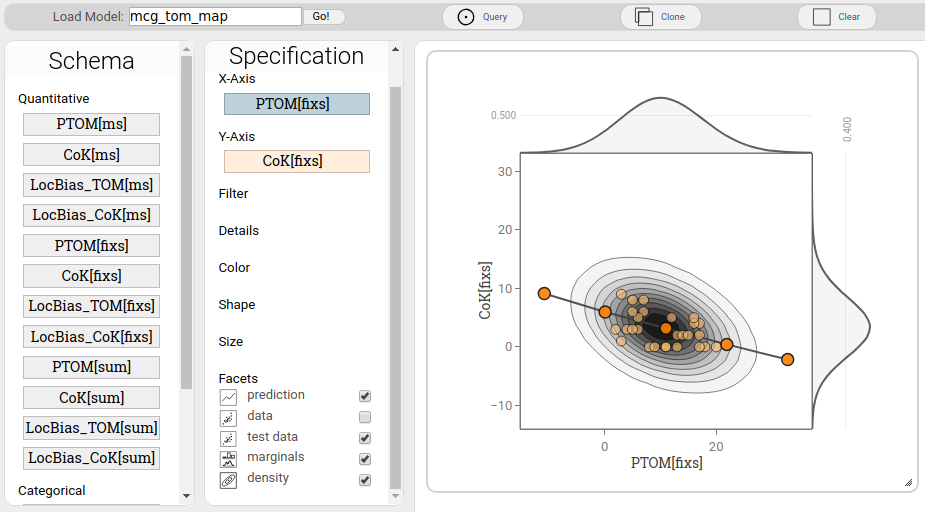
\includegraphics[width=\textwidth]{images/lumen_screenshot.png}
	\caption{View on the lumen frontend}
	\label{fig:lumen_screenshot}
\end{figure}
After a model is loaded, all random variables of the model are shown in the 'Schema'-panel on the left. A user then has to select the variables that should be displayed by dragging the according names into the 'Specification'-panel in the middle. There, a choice has to be made on which channel the information of a variable should be displayed. The available channels are:
\begin{itemize}
	\item X-Axis
	\item Y-Axis
	\item Color
	\item Shape
	\item Size
\end{itemize}
Once one or more variables are moved there, the according visualization is shown in the right panel. Additionally, a filter can be set to only consider a specified interval within the range of a variable. The user can also select which elements of the model should be displayed. The following elements can be chosen:
\begin{itemize}
	\item prediction
	\item data
	\item test data
	\item marginals
	\item density
\end{itemize}
For the prediction, it is possible to specify any of the selected variables as dependent or independent. It is also possible to specify additional independent variables for the prediction by dragging them into the 'Details' field.
\\
Visualizing a model as described above can require marginalizing and conditioning it multiple times. The necessary operations are performed by the modelbase backend \cite{Lucas2016b}. How modelbase was complemented to enable a visualization of models built with PyMC3 is described in \autoref{sec:lumen_pymc3_integration}.

%A model class is described by a python file that includes a class with several prescribed methods.

%stochastic data types (--> probability distributions) make it easier to perform Bayesian data analysis
%Random Variables can be represented as objects

%model classes are in \url{modelbase/mb_modelbase/models_core}
%data is in \url{mb_data}. model fitting is done in the script fit\_models.py, which is also in \url{mb_data}. The corresponding model class has to be imported, the models have to be 'registered' in the known\_models variable and then the models to be fit have to be listed in the variable debugincl.

%Fitted models that can be accessed by lumen are then stored in \url{data_models}.

%In the mb\_data repository, data that can be used for model fitting is contained. It has a file named fit\_models.py that contains specifications of data and corresponding models. It can be called with one of these specifications to create a mdl file. In the directory data\_models all mdl files are currently stored that can be displayed by the lumen frontend.

\section{Example: Building a probabilistic model}
\label{sec:Comparison}
\textit{To check if PyMC3 is applied correctly, I fit a Bayesian model first without the use of a PPL. Then I fit the same model by using PyMC3. The results of both approaches are compared.}
\\
Assume we want to fit a model with the two dimensions $x$ and $mu$, one of them, $x$, we can observe, the other one, $mu$, we can't observe. Furthermore, we assume the following priors:
\begin{equation}
\begin{split}
mu &\sim N(0,1)\\
x &\sim N(mu,1)
\end{split}
\end{equation}
Assume again, that we observe some data $X$ of the observable dimension $x$.
We now want to compute the joint posterior distribution of both dimensions $mu$ and $x$, conditioned on the observed data $X$.
\\
The data $X$ is generated as follows:\\
\begin{figure}[h]
	\begin{lstlisting}
	# Generate data
	numpy.random.seed(1)
	size = 100
	mu = numpy.random.normal(0,1,size=size)
	sigma = 1
	X = numpy.random.normal(mu,sigma,size=size)
	
	\end{lstlisting}
	\label{fig:groundtruth_example_code_data_generation}
\end{figure}
\subsection{Creating a simple Bayesian model without PyMC3}
\label{subsec: Complete example of a simple Bayesian model}

The joint posterior distribution is computed as shown in \autoref{eq:jointposterior}.
\begin{equation}
\label{eq:jointposterior}
\begin{split}
&P(x,mu|X) \\
= &P(x|mu,X) * P(mu|X) \\
= &P(x|mu) * P(mu|X) \\
= &P(x|mu) * P(X|mu) * P(mu) / P(X) \\
= &P(x|mu) * P(X|mu) * P(mu) / \int P(X,mu) \hspace{1mm} d \hspace{1mm} mu \\
= &P(x|mu) * P(X|mu) * P(mu) / \int P(X|mu) * P(mu) \hspace{1mm} d \hspace{1mm} mu
\end{split}
\end{equation}
Each element of the last line of \autoref{eq:jointposterior} can be implemented in Python relatively easy: 
\\
The likelihood for any new data point given $mu$, $P(x|mu)$, is, according to our model assumptions, the density of $x$ in a normal distribution with mean $mu$. It can be be implemented as shown in \autoref{fig:likelihood_new_data_point}.
\begin{figure}[h]
	\begin{lstlisting}
	from scipy.stats import norm
	def likelihood_x(x,mu):
	density = norm.pdf(x, loc=mu, scale=1)
	return density
	\end{lstlisting}
	\caption{Implementation of the likelihood for one data point}
	\label{fig:likelihood_new_data_point}
\end{figure}
\\
The likelihood of the observed data $X$ given $mu$, $P(X|mu)$, is the product of the likelihoods for each data point in $X$. It can be implemented as shown in \autoref{fig:likelihood_observed_data}.
\begin{figure}[h]
	\begin{lstlisting}
	def likelihood_X(X,mu):
	res = 1
	for point in X:
	res *= likelihood_x(point,mu)
	return res
	\end{lstlisting}
	\caption{Implementation of the likelihood for the observed data}
	\label{fig:likelihood_observed_data}
\end{figure}
\\
The prior probability for any $mu$, $P(mu)$, is just the density of the standard normal distribution at the point $mu$, as shown in \autoref{fig:prior_mu}:
\begin{figure}[h]
	\begin{lstlisting}
	def prior_mu(mu):
	density = norm.pdf(mu, loc=0, scale=1)
	return density
	\end{lstlisting}
	\caption{Implementation of the prior for mu}
	\label{fig:prior_mu}
\end{figure}
The last part of the equation, the integral of the product between likelihood and prior, is computationally more intensive but nevertheless easy to implement as well. \autoref{fig:prior_X} shows the implementation.
\begin{figure}[h]
	\begin{lstlisting}
	def likelihood_times_prior_mu(X,mu):
	return likelihood_X(X,mu) * prior_mu(mu)
	
	def prior_X(X):
	res = integrate.quad(
	lambda mu: likelihood_times_prior_mu(X,mu),a=-np.inf,b=np.inf)[0]
	return res
	\end{lstlisting}
	\caption{Implementation of the prior for X}
	\label{fig:prior_X}
\end{figure}
\\
At last, we only have to multiply all those pieces to get to a posterior joint density for any combination of $X$ and $mu$. \autoref{fig:joint_posterior} shows the according implementation.
\begin{figure}[h]
	\begin{lstlisting}
	def joint_posterior(x,mu,X):
	res = likelihood_x(x,mu) * likelihood_X(X,mu) * prior_mu(mu) / prior_X(X)
	return res
	\end{lstlisting}
	\caption{Implementation of the joint posterior distribution}
	\label{fig:joint_posterior}
\end{figure}
\\
The joint posterior distribution can now be visualized as it is done in \autoref{fig:ground_truth_posterior_1}.
\begin{figure}
	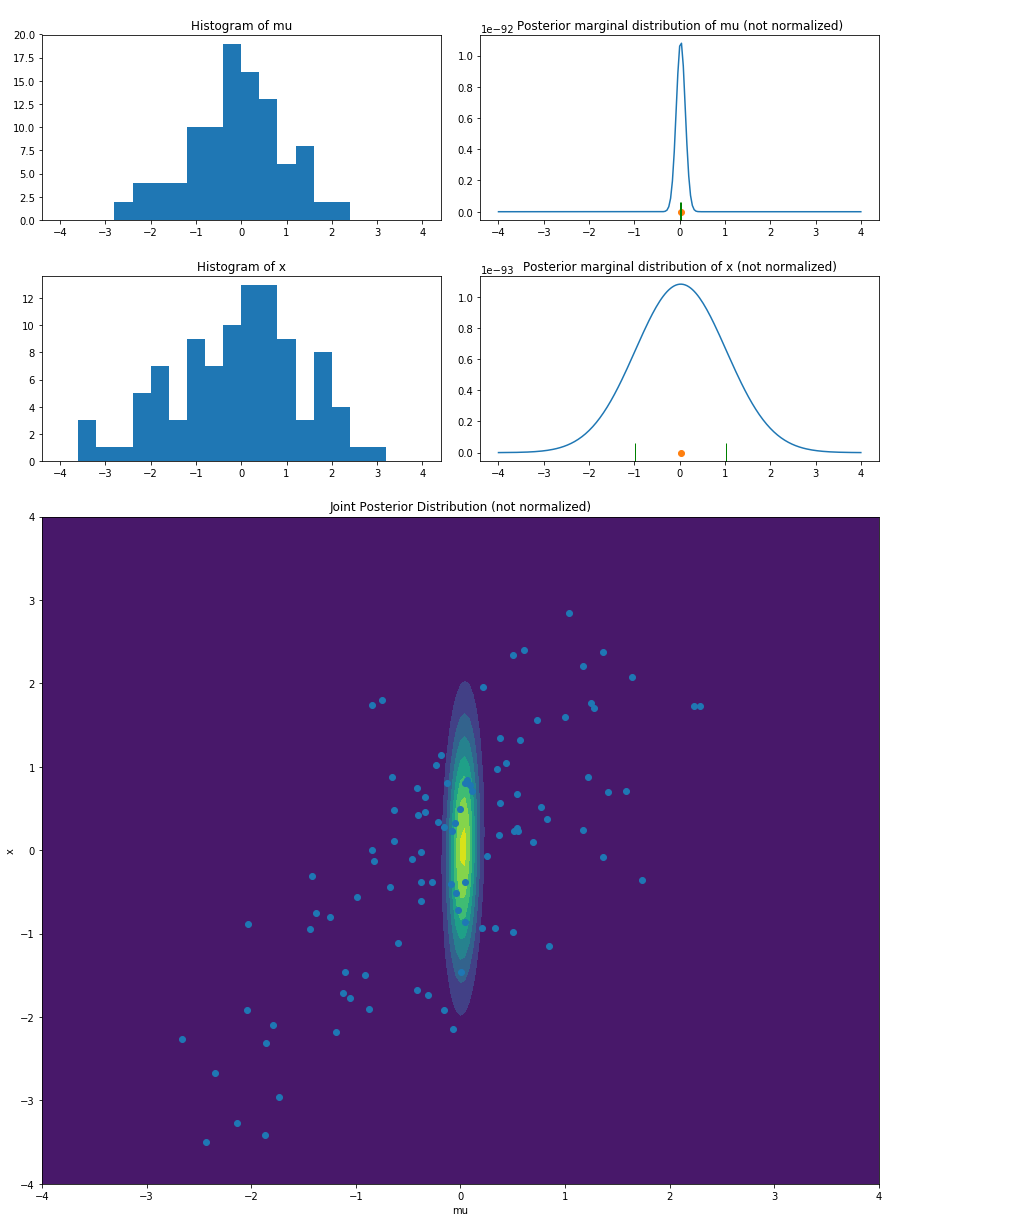
\includegraphics[width=\textwidth]{images/ground_truth_posterior_1_cut.png}
	\caption[Posterior distributions of the example model]{Posterior distributions of the example model}
	\label{fig:ground_truth_posterior_1}
\end{figure}
The upper left figures show histograms of the data points of $x$ and $mu$. The upper right figures show the marginalized posterior distributions for both variables. The bottom figure shows the density of the joint posterior distribution as a contour plot, along with the data points. We see that $mu$ is very narrowly contained around zero whereas $x$ has a much broader distribution. A relationship between $mu$ and $x$ is not visible. This is astonishing at first: Since we know that $x$ is dependent on $mu$, I would expect this dependency to show up in the visualization. In other words, I would expect the probability density for a high $mu$ and a high $x$ to be relatively similar to the density of a $mu$ near zero and a high $x$, and to be much higher than the density of a high $mu$ and a low $x$.
Let's look again at the formula:
\begin{equation}
P(x,mu|Y) = P(x|mu) * P(X|mu) * P(mu) / \int P(X|mu) * P(mu) \hspace{1mm} d \hspace{1mm} mu
\end{equation}
To evaluate the above mentioned expectations, it is not necessary to keep the normalizing constant since it does not affect the order of the values. So we keep:
\begin{equation}
P(x,mu|Y) = P(x|mu) * P(X|mu) * P(mu)
\end{equation}
When we consider only the first and the last term of from the right of this formula, it behaves exactly as expected: \begin{equation}
P(x=high|mu=high)*P(mu=high) = P(x=high|mu=zero)*P(mu=zero)
\end{equation}
and 
\begin{equation}
P(x=high|mu=high)*P(mu=high) >> P(x=low|mu=high)*P(mu=high)
\end{equation} What was messing with the expectations is the term in the middle which gives the likelihood of the observed data. For a value of $mu$ that is far from the true mean, that term quickly becomes extremely small since all the data points speak against it. That's why the distribution is so strongly centered to the middle: All the outer values of $mu$ are getting assigned extremely low density values by this middle term. 
%I still don't quite understand why it is centered \textit{that} strong: The real $mu$ is distributed far wider, with a standard deviation of 1.
The dependence between $mu$ and $x$ is in fact still there in the joint posterior distribution, it's just overlapped by the centering effect of the data. To understand this example better, I make changes in the model and/or in the data generation and look how those changes affect the posterior distributions. Firstly, the model is learned without any data points. It delivers the distribution that is shown in \autoref{fig:ground_truth_posterior_5}.
\begin{figure}
	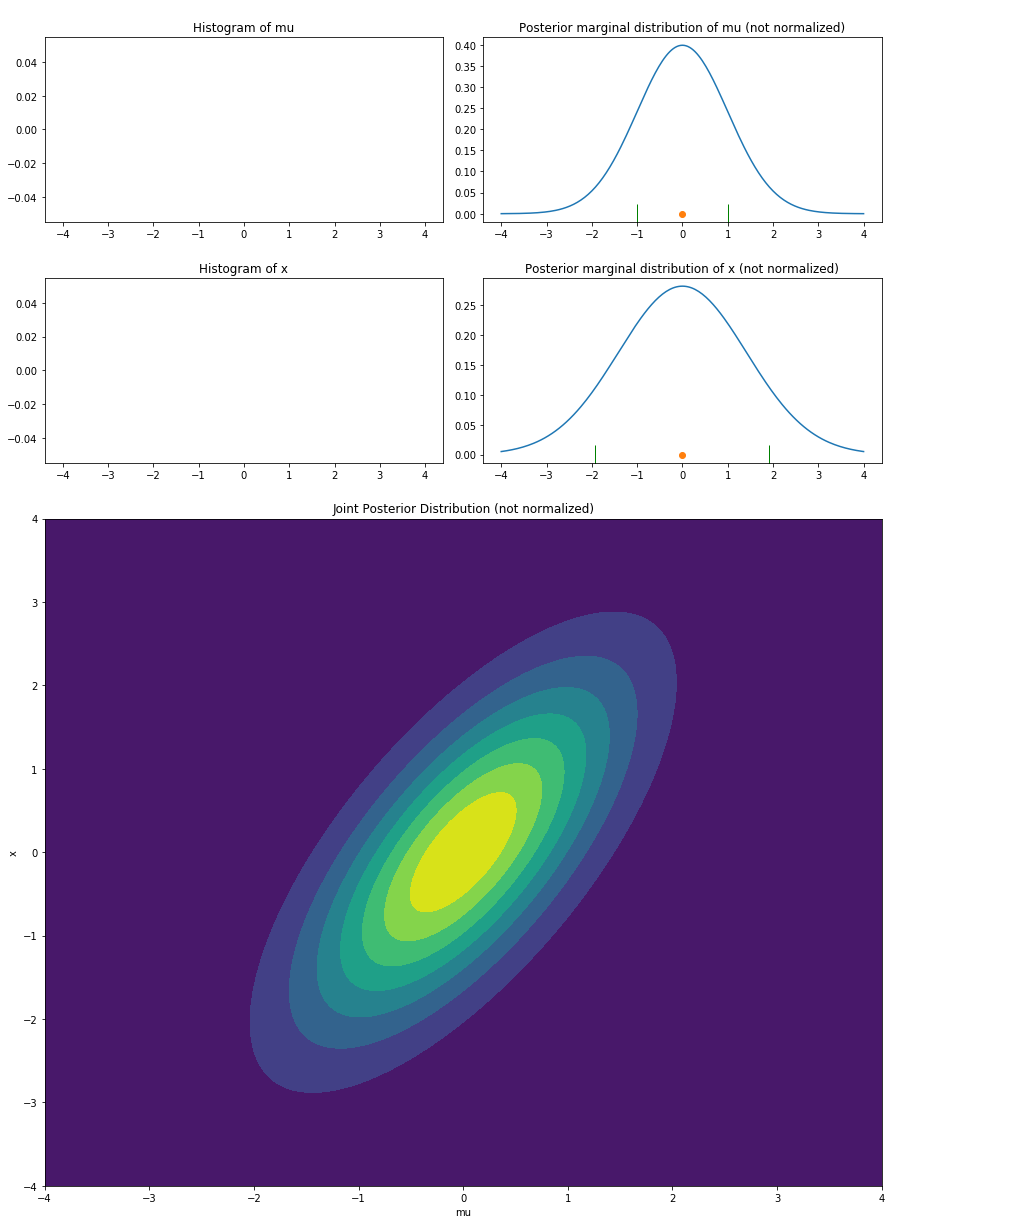
\includegraphics[width=\textwidth]{images/ground_truth_posterior_5_cut.png}
	\caption[Posterior probability densities of the example model without any data points]{Posterior probability densities of the example model without any data points}
	\label{fig:ground_truth_posterior_5}
\end{figure}
The dependency between the variables is here clearly visible since the data points do not influence the plot anymore. The more data points we include, the more the joint posterior distribution is compressed to the center, as shown in \autoref{fig:posterior_different_data_sizes}.
\begin{figure}
	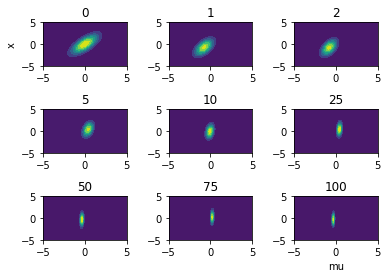
\includegraphics[width=\textwidth]{images/posterior_different_data_sizes.png}
	\caption[Posterior distributions for different numbers of data points]{Posterior distributions for different numbers of data points}
	\label{fig:posterior_different_data_sizes}
\end{figure}
When the variance in both the data generation and the prior for mu increases: the data will be more spread. I expect the $P(X|mu)$-part of the joint posterior to not change, since the data $X$, on the one hand, will be more spread out, which is in favor of smaller density values, but on the other hand, the variance of the prior distribution is also higher, which leads to bigger density values for points far from the mean. The $P(x|mu)$-part will probably contribute to a wider distribution in both dimensions: $P(x|mu)$ for a given $x$ gets assigned a lower probability value in the center and bigger values on the edges, when increasing the variance. The same is true for a given $mu$. The $P(mu)$-part will also contribute to a wider distribution in the $mu$-dimension.
So when increasing the variance, I expect the whole distribution to get wider, especially in the $mu$-direction.
\\
What happens: when choosing a standard deviation of 5, the density is always zero. This is likely due to numerical difficulties, since the values computed here are very small.
I can set the number of data points down, then we get densities different from 0.
\\
\autoref{fig:ground_truth_posterior_3} and \autoref{fig:ground_truth_posterior_4} show a comparison between a posterior distribution where the parameter for the standard deviation in the data generation and in the prior is set to 1, and a posterior distribution where this parameter is set to 5. Astonishingly, the standard deviation of the posterior is nearly the same in both cases whereas the mean of the variables in the latter distribution is at around -1.5. I don't know yet why this happens. 
\begin{figure}
	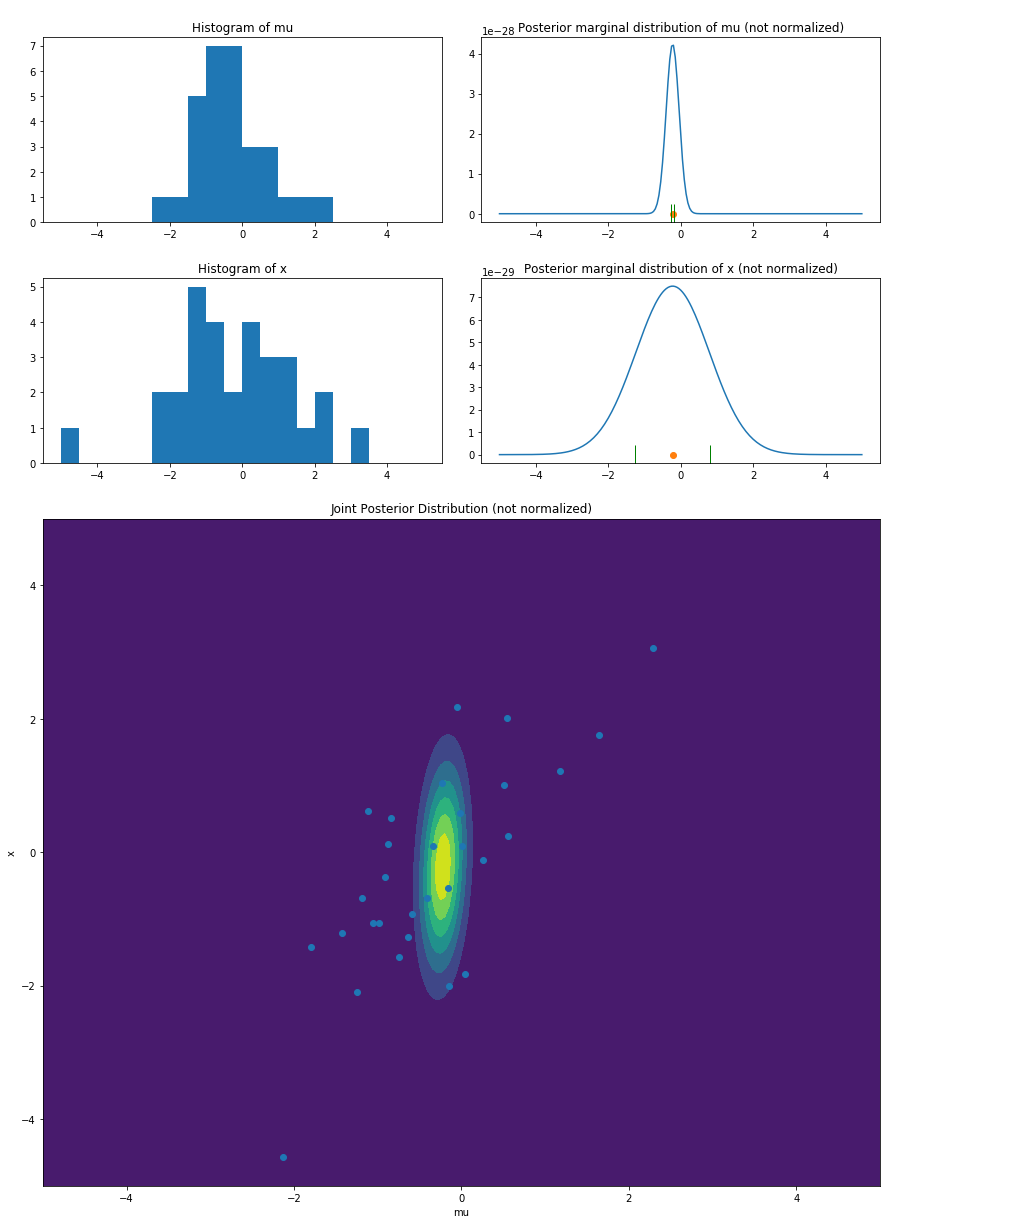
\includegraphics[width=\textwidth]{images/ground_truth_posterior_3_cut.png}
	\caption[Posterior probability densities of the example model with standard deviation of 1]{Posterior probability densities of the example model with standard deviation of 1}
	\label{fig:ground_truth_posterior_3}
\end{figure}
\begin{figure}
	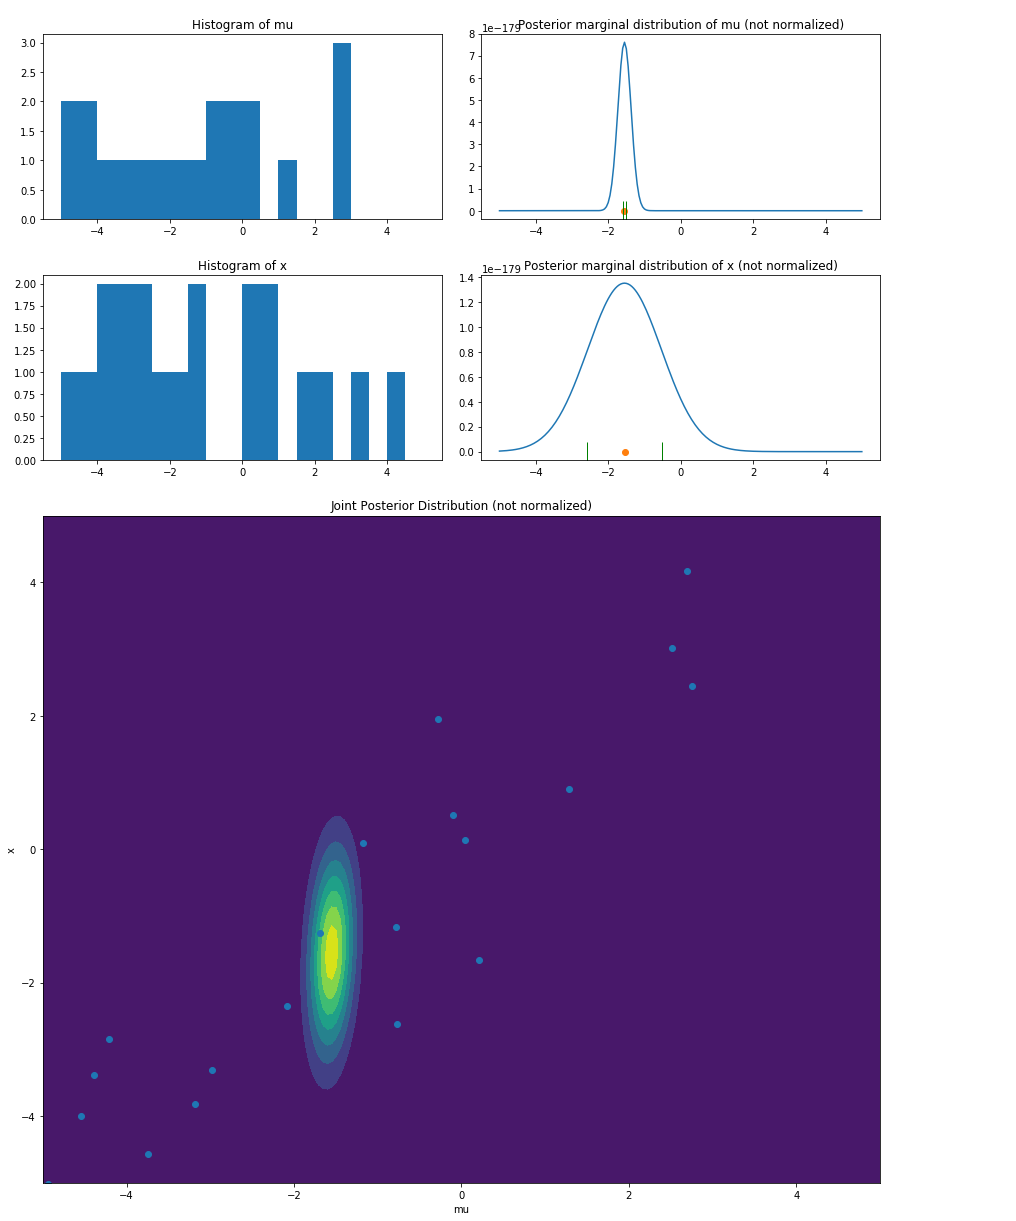
\includegraphics[width=\textwidth]{images/ground_truth_posterior_4_cut.png}
	\caption[Posterior probability densities of the example model with standard deviation of 5]{Posterior probability densities of the example model with standard deviation of 5}
	\label{fig:ground_truth_posterior_4}
\end{figure}
%When the number of actual data points becomes small, I expect %the joint distribution to show the linear relationship between %$x$ and $mu$ better, since the influence of the data points, %which 'compresses' the whole plot to the middle, diminishes.

%This is also what actually happens. Without any data points, we %see clearly the linear relationship.

When we change the data generating mechanism to a non-hierarchic process so that only a single variable is drawn from a normal distribution with mean 0 and the combined standard deviation from the previous two variables, I expect a similar posterior distribution as before. I've not found out yet if there is a parameterization for a normal distribution that generates the same data as the hierarchical model described here. So far as I can tell, the data produced by the non-hierarchic process should look different than the data produced by the hierarchic process. This makes me expect the posterior calculated by using data from such a non-hierarchical model look at least slightly different from the hierarchical case. However, as one can see in \autoref{fig:ground_truth_posterior_6}, the distribution looks very similar. At this point I cannot tell if the differences introduced by the change in data generation are actually very small, or if the posterior distributions are really the same apart from random errors, and there is either an error in the code or in my thinking.
\begin{figure}
	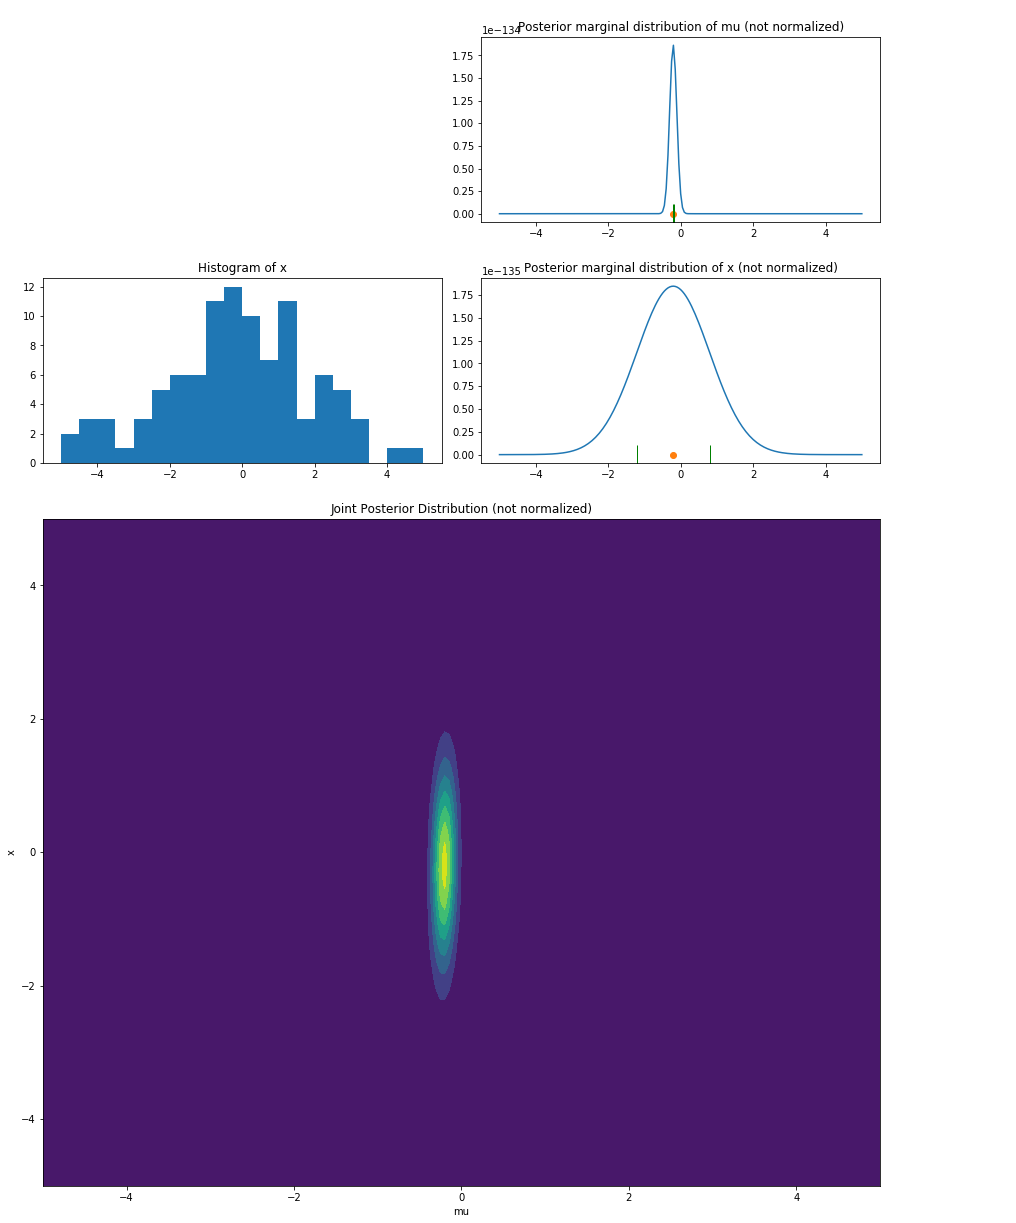
\includegraphics[width=\textwidth]{images/ground_truth_posterior_6_cut.png}
	\caption[Posterior probability densities of the example model with altered data generation]{Posterior probability densities of the example model with altered data generation}
	\label{fig:ground_truth_posterior_6}
\end{figure}
If it is possible to generate the same data by different parametrizations, it means that a model cannot be able to always return the true parameters in the posterior. This is also called Nonidentifiability.
\subsection{PyMC3 example of a simple Bayesian model}
\label{subsec: PyMC3 example of a simple Bayesian model}
The model from \autoref{subsec: Complete example of a simple Bayesian model} is now created by using PyMC3 with the code shown in \autoref{fig:PyMC3_example_code_simple_model}.
\begin{figure}[h]
	\begin{lstlisting}
	import numpy as np
	import pandas as pd
	import pymc3 as pm
	import matplotlib.pyplot as plt
	
	# Generate data
	np.random.seed(2)
	size = 100
	mu = np.random.normal(0,1,size=size)
	sigma = 1
	X = np.random.normal(mu,sigma,size=size)
	
	# Specify model
	basic_model = pm.Model()
	with basic_model:
	sigma = 1
	mu = pm.Normal('mu',mu=0,sd=sigma)
	X = pm.Normal('X',mu=mu,sd=sigma,observed=X)
	
	# Draw samples from posterior
	nr_of_samples = 100
	with basic_model:
	trace = pm.sample(nr_of_samples,chains=1)
	samples_mu = trace['mu']
	samples_X = np.random.normal(samples_mu,1,size=nr_of_samples)
	\end{lstlisting}
	\caption[Code used to specify the example model in PyMC3]{Code used to specify the example model in PyMC3}
	\label{fig:PyMC3_example_code_simple_model}
\end{figure}
First, the same data is generated as in \autoref{subsec: Complete example of a simple Bayesian model}. Then, $mu$ and $X$ are specified, $mu$ as a stochastic random variable and $X$ as an observed stochastic random variable. Finally, samples from the posterior distribution are drawn using the sample-method. TODO: use a PyMC3-method to draw samples from $X$.
Figure \ref{fig:PyMC3_joint_posterior_samples_simple_model} shows these samples. Similarities in shape to the real joint posterior distribution in \autoref{fig:ground_truth_posterior_1} are visible, so it is assumed that PyMC3 captures the model correctly.
\begin{figure}
	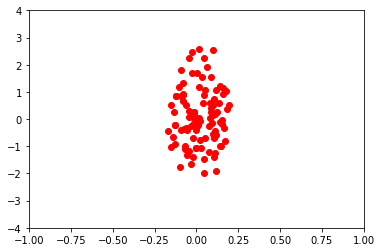
\includegraphics[width=\textwidth]{images/PyMC3_joint_posterior_samples_simple_model.png}
	\caption[Samples from the posterior joint distribution of the example model in PyMC3]{Samples from the posterior joint distribution of the example model in PyMC3}
	\label{fig:PyMC3_joint_posterior_samples_simple_model}
\end{figure}

\section{Integration of PyMC3 in Lumen}
\label{sec:lumen_pymc3_integration}
Visualizing a model as described in \autoref{sec:Lumen} can require marginalizing and conditioning it multiple times. The necessary operations are performed by the modelbase backend. In it, each model type is represented by a class. This class is required to provide certain methods that allow to manipulate the model in a way that proper data can be generated for the frontend. The most important operations that are embedded in these methods are:
\begin{itemize}
	\item fitting a model
	\item marginalization
	\item conditioning
	\item computing the probability density for a given data point
\end{itemize}
Visualizing models built with PyMC3 in Lumen requires the abovementioned operations to be carried out for those models. Expanding Lumen by implementing these operations for arbitrary models poses the main task of the thesis at hand. Below is explained how this was done for each of these operations.
\paragraph{Fitting a model} in Bayesian statistics means finding the joint posterior distribution. In the context of Probabilistic Programming, it means drawing samples from all random variables so that the joint posterior distribution can be approximated. PyMC3 provides methods for sampling from both observed and unobserved random variables which only have to be applied here. Figure \ref{fig:code_fitting_a_model} shows my implementation of the process. There, the variable $self.model\_structure$ holds the full model that was created before in PyMC3. As an additional feature, since in Bayesian data analysis there is no test data, the samples that were generated during the fitting process are assigned to the variable that originally was supposed to hold the test data. This way, the sample points can later be visualized in Lumen, albeit to some extent incorrectly labeled as test data.
\begin{figure}[h]
	\begin{lstlisting}
	import pymc3 as pm
	def _fit(self):
	with self.model_structure:
	# Draw samples
	nr_of_samples = 500
	trace = pm.sample(nr_of_samples,chains=1,cores=1)
	for varname in trace.varnames:
	self.samples[varname] = trace[varname]
	ppc = pm.sample_ppc(trace)
	for varname in self.model_structure.observed_RVs:
	# each sample has 100 draws in the ppc, so take only the first one for each sample
	self.samples[str(varname)] = [samples[0] for samples in np.asarray(ppc[str(varname)])]			
	# Change order of sample columns so that it matches order of fields
	self.samples = self.samples[self.names]
	self.test_data = self.samples
	return ()
	
	\end{lstlisting}
	\caption[Implementation of fitting a model]{Implementation of fitting a model}
	\label{fig:code_fitting_a_model}
\end{figure}

\paragraph{Marginalizing a model} normally means that one has to integrate over the variables that should be removed. In the case of Probabilistic Programming where we have only samples instead of analytical functions, it is far easier: The samples of the variables one wants to marginalize out are just removed and that's it. The corresponding code is shown in \autoref{fig:code_marginalizing_a_model}.
\begin{figure}[h]
	\begin{lstlisting}
	def _marginalizeout(self, keep, remove):
	# Remove all variables in remove
	for varname in remove:
	if varname in list(self.samples.columns):
	self.samples = self.samples.drop(varname,axis=1)
	return ()
	
	\end{lstlisting}
	\caption[Implementation of marginalizing a model]{Implementation of marginalizing a model}
	\label{fig:code_marginalizing_a_model}
\end{figure}

\paragraph{Conditioning a model} follows the same principle as marginalizing: Samples that do not fall inside the interval dictated by the condition are just removed. This operation is implemented as shown in \autoref{fig:code_conditioning_a_model}.
\begin{figure}[h]
	\begin{lstlisting}
	def _conditionout(self, keep, remove):
	names = remove
	fields = self.fields if names is None else self.byname(names)
	# Here: Konditioniere auf die Domaene der Variablen in remove
	for field in fields:
	# filter out values smaller than domain minimum
	filter = self.samples.loc[:,str(field['name'])] > field['domain'].value()[0]
	self.samples.where(filter, inplace = True)
	# filter out values bigger than domain maximum
	filter = self.samples.loc[:,str(field['name'])] < field['domain'].value()[1]
	self.samples.where(filter, inplace = True)
	self.samples.dropna(inplace=True)
	return ()
	\end{lstlisting}
	\caption[Implementation of conditioning a model]{Implementation of conditioning a model}
	\label{fig:code_conditioning_a_model}
\end{figure}

\paragraph{Getting a probability density} in the context of Probabilistic Programming is not as straightforward as in classical statistics since we do not have probability density function. This function instead can be approximated by the samples drawn from the posterior. In the implementation at hand, the chosen approximation method is the kernel density estimation using Gaussian kernels, provided by the scikit-learn package \cite{scikit-learn}. In this method, each data point is assigned a Gaussian curve centered on the point. The density for a given point is then determined by summing up the densities of all the Gaussians. It is implemented as shown in \autoref{fig:code_probability_density}.
\begin{figure}[h]
	\begin{lstlisting}
	def _density(self, x):
	X = self.samples.values
	kde = KernelDensity(kernel='gaussian', bandwidth=0.1).fit(X)
	x = np.reshape(x,(1,len(x)))
	logdensity = kde.score_samples(x)[0]
	return np.exp(logdensity).item()
	\end{lstlisting}
	\caption[Implementation of computing the probability density for a given point]{Implementation of computing the probability density for a given point}
	\label{fig:code_probability_density}
\end{figure}

\paragraph{Treating independent variables}
Displaying independent variables currently is not supported in Lumen.

%Another method is the one that marginalizes a random variable out. In a Bayesian model, a random variable can be a parameter as well as a data dimension.  What is wanted here is thus the posterior distribution over all variables listed in keep.
%In PyMC3, marginalizing means sampling over a subset of the variables. Samples were already drawn in the fitting method, so only the corresponding columns of those samples have to be chosen here.
%The marginal density plots of mu from the basic manual example looked different than the marginal plots of mu in lumen. Part of the reason for this is the Gaussian kernel density estimation. If the bandwidth parameter is too high, it has a smoothing effect that lets the plot look different than the one in the basic manual example. Setting the bandwidth to 0.1 removed this difference. Although the shape of the marginal plots is now similar, the absolute values are still very different. For a mu of 0, the density of the basic manual example is about 4.0, whereas in lumen it is at about 0.13. Which one is correct??
%First Bug in the model run: Beim Laufen der Skripte für Lumen wir die Marginalisierungsmethode mit den Datendimensionen als Parameter angewendet. Meine erste Implementierung lässt aber nur Marginalisierungen auf Parameter zu, dadurch gibt es einen Fehler.
%Second Bug in the model: The marginalization method needs to access all variables of the data. However, it gets only the data passed for those variables to keep. So it cannot access the other variables. 
%Problem: Model data is reduced to variables in keep. Lösungsidee: Setze zu Beginn der Methode die Daten auf den vollständigen Datensatz, und setze am Ende der Methode die Daten wieder auf die Dimensionen in keep zurück.
%Problem: Es ist nicht gut, dass bei jedem Aufruf der \_density-Methode gesampelt wird, da das viel Zeit und Speicher braucht. Lösung: Führe das Sampling nur einmal durch und speichere die samples in einer Klassenvariable.

\section{Example Cases}

\textit{In this chapter, case examples are presented to show how the finished interface performs in practice.}

\subsection{First simple example}
As a basic example to implement in PyMC3 we choose the model from \autoref{subsec:Comparison}. The expectation here is that the resulting Lumen plot should look much like the visualizations in \autoref{fig:code_use_case_1}. The model contains the random variables $X$ and $mu$, the data for it was generated by the following  distributions:
\begin{equation}
\begin{split}
X &\sim N(\mu,1), \\
\mu &\sim N(0,1),
\end{split}
\end{equation}
The priors for $X$ and $mu$ match exactly these distributions. The corresponding model is described in PyMC3 as shown in \autoref{fig:code_use_case_1}.
\begin{figure}[h]
	\begin{lstlisting}
    basic_model = pm.Model()
	with basic_model:
		mu = pm.Normal('mu', mu=0, sd=1)
		X = pm.Normal('X', mu=mu, sd=1, observed=data['X'])
	\end{lstlisting}
	\caption[PyMC3 model of use case 1]{PyMC3 model of use case 1}
	\label{fig:code_use_case_1}
\end{figure}
Visualizing this model in Lumen results in the plot shown in \autoref{fig:lumen_use_case_1}. Considering the different ranges in the $mu$-axis, the plot looks quite similar to the visualizations in \autoref{fig:ground_truth_posterior_1}, meeting the expectations.
\begin{figure}
	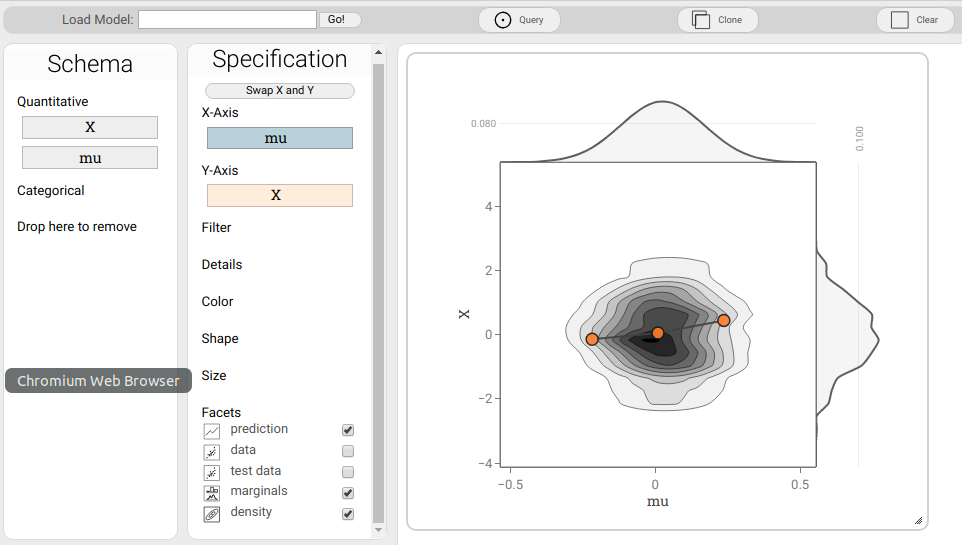
\includegraphics[width=\textwidth]{images/lumen_use_case_1.png}
	\caption{Lumen visualization of use case 1}
	\label{fig:lumen_use_case_1}
\end{figure}
\subsection{Linear Regression}
As another basic use case, a linear regression model used by Salvatier et al to illustrate the PyMC3 functionality \cite{Salvatier2016}, is visualized. 
The model is explained by Salvatier et al as follows:\\
"We are interested in predicting outcomes $Y$ as normally-distributed observations with an expected value $mu$ that is a linear function of two predictor variables, $X_1$ and $X_2$:
\begin{equation}
\begin{split}
Y &\sim N(\mu,\sigma^2), \\
\mu &= \alpha + \beta_1 X_1 + \beta_2 X_2
\end{split}
\end{equation}
where $\alpha$ is the intercept, and $\beta_i$ is the coefficient for covariate $X_i$, while $\sigma$ represents the observation or measurement error."\\
The following priors are assigned to the random variables:
\begin{equation}
\begin{split}
\alpha &\sim N(0,10), \\
\beta_1 &\sim N(0,10), \\
\beta_2 &\sim N(0,10), \\
\sigma &\sim |N(0,1)|
\end{split}
\end{equation}
The code creating this model is shown in \autoref{fig:code_use_case_2}. It differs from the implementation of Salvatier et al in that the variables $X_1$ and $X_2$ are also treated as random variables. This change was made since we want to display these variables in Lumen, and Lumen currently can only display random variables.
\begin{figure}[h]
	\begin{lstlisting}
	np.random.seed(123)
	alpha, sigma = 1, 1
	beta_0 = 1
	beta_1 = 2.5
	size = 100
	X1 = np.random.randn(size)
	X2 = np.random.randn(size) * 0.2
	Y = alpha + beta_0 * X1 + beta_1 * X2 + np.random.randn(size) * sigma
	data = pd.DataFrame({'X1': X1, 'X2': X2, 'Y': Y})
	
	basic_model = pm.Model()
	with basic_model:
	     # Priors for unknown model parameters
	     alpha = pm.Normal('alpha', mu=0, sd=10)
	     beta_0 = pm.Normal('beta_0', mu=0, sd=10)
	     beta_1 = pm.Normal('beta_1', mu=0, sd=10)
	     sigma = pm.HalfNormal('sigma', sd=1)
	
	     # Expected value of outcome
	     mu = alpha + beta_0 * data['X1'] + beta_1 * data['X2']
	
	     # Likelihood (sampling distribution) of observations
	     Y = pm.Normal('Y', mu=mu, sd=sigma, observed=data['Y'])
	     X1 = pm.Normal('X1', mu=data['X1'], sd=sigma, observed=data['X1'])
	     X2 = pm.Normal('X2', mu=data['X2'], sd=sigma, observed=data['X2'])
	\end{lstlisting}
	\caption[PyMC3 model of use case 2]{PyMC3 model of use case 2}
	\label{fig:code_use_case_2}
\end{figure}
\\
TODO: The model does not at all match the data. Either change the model so that it matches or make the reasoning more consistent, why I want a model that does not fit well.
\subsection{Eight schools model}
The problem shown below is often used in the literature as an example to illustrate Bayesian modeling \cite{1439840954}\cite{sinharay2003posterior}\cite{rubin1981estimation}. It is about eight schools where the impact of a coaching program on test results was estimated. For each school a separate estimate and a standard error was calculated. These estimates are shown in \autoref{fig:eightschools_data} and serve as data for our modeling problem.\\ 
Sinhara et al now fit a hierarchical model for this process and apply a number of methods to check in which ways their models deviates from the data \cite{sinharay2003posterior}. Below, their methods are recapitulated and it is analyzed if the conclusions they draw can also be deduced from a visualization of the model in Lumen.
\begin{figure}
	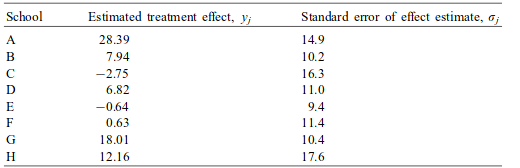
\includegraphics[width=\textwidth]{images/eightschools_data.png}
	\caption[Observed effects and standard errors of coaching programs on test scores in 8 schools. Source: \cite{sinharay2003posterior}]{Observed effects and standard errors of coaching programs on test scores in 8 schools}
	\label{fig:eightschools_data}
\end{figure}
Sinharay et al use a hierarchical normal-normal model shown in \autoref{eq:eightschools_model} to capture the mechanism: An estimated treatment effect $y_i$ is there seen as an independent draw from a normal distribution that is centered around the real treatment effect $\theta_i$. However, it is assumed that each school potentially has a different treatment effect which, in turn, is independently drawn for every school from the same normal distribution. The mean $\mu$ and the standard deviation $\tau$ of this normal distribution are hyperparameters with uniform priors.
\begin{equation}
\label{eq:eightschools_model}
\begin{split}
y_i &\sim N(\theta_i,\sigma_i),\\
\theta_i &\sim N(\mu,\tau), \\
\mu &\sim 1, \\
\tau &\sim 1, \\
&i=1,...,8
\end{split}
\end{equation}
Simulations from posterior distributions were obtained for $\tau$, $\mu$ and $\theta$ by finding the conditional distributions $p(\tau|\textit{y})$, $p(\mu|\tau, \textit{y})$ and $p(\theta|\tau, \mu, \textit{y})$ and then sampling from these distributions, where $\textit{y}$ denotes the observed estimated treatment effects. For each draw from those distributions, eight data points $y^{rep}$ were generated and a number of test statistics was calculated on them: the largest of the eight observed outcomes,  the smallest of the eight observed outcomes,the  average, and the sample  standard deviation. Those test statistics were then displayed graphically and compared to the according test statistic of the observed effects $\textit{y}$.\\
This is not possible in the Lumen setup: For one, it is not possible to display summary statistics, only actual observed data. Second, samples there are drawn from the joint posterior distribution of all variables. We can't draw hierarchically from the joint posterior of a subset of variables, and then generate a number of samples for the rest of the variables.
\autoref{fig:eightschools_lumen_vis} shows the visualization of the coaching effects in lumen. It looks not very informative, for one because there is so few data (it only shows four instead of eight data points because it is split in training and testing data in advance, and only displays the training data), and second because the plot is fragmentized into many small peaks.
\begin{figure}
	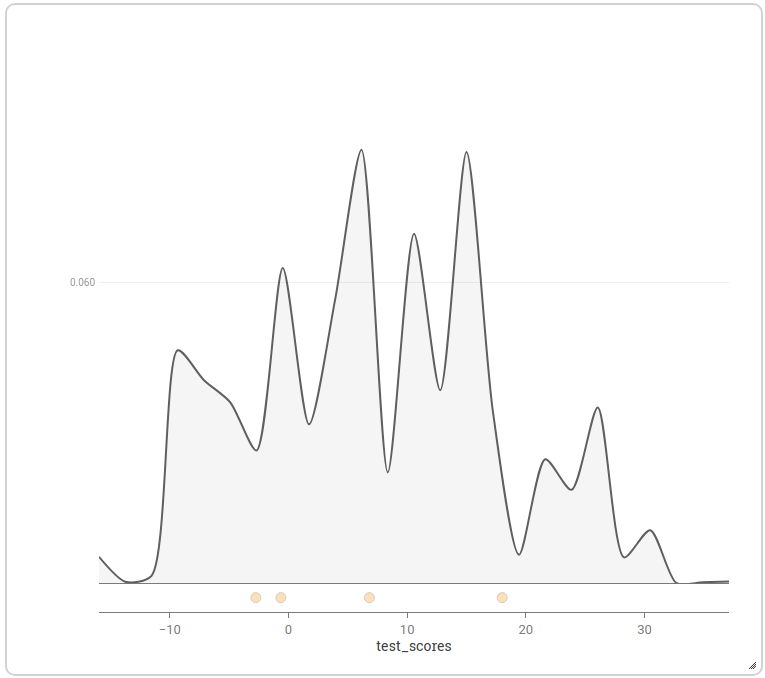
\includegraphics[width=\textwidth]{images/eight_schools_lumen_vis.png}
	\caption[Visualization of the coaching effects for the eight schools model in Lumen]{Visualization of the coaching effects for the eight schools model in Lumen}
	\label{fig:eightschools_lumen_vis}
\end{figure}
TODO: More data points into the plot and see how the lumen visualization looks then.
%\\
%Sinharay et al find that their simulated statistics overall fit well to the observed statistics, only the standard deviation is higher in the simulated values than in the observed ones.\\
%In Lumen, comparing the model to the data for this particular model is difficult since we only have so few data points. A statement how well the data fits to the model, cannot be made.\\
%Next, Sinharay et al simulate $\theta$ with a fixed $\mu$ and a fixed $\tau$ for different numbers of schools: 8,16,50 and 100. Then $y$ is simulated with different fixed numbers of $\sigma^2$:1,20,168. and then do the same checks as above. They do not display it graphically this time, probably because of the bigger number of combinations, but give the percentiles of the p-values instead. TODO: Understand that part.
%Sinharay et al then fit a different model with an exponential rather than a uniform prior, do the tests again, and find that only some of them give worse results in the second model, as they should, since the model is false. 

 \section{Discussion}
More complex models
Visualizing models that are used in practice by PPL users.
How can the Lumen visualization help PPL uses to deal with their models?
Summaries can't be visualized, e.g. residuals

from Gelman and others recommended approach: Compare observed data to simulated data. Lumen approach: Compare observed data to joint posterior probability density.


\section {Conclusion}
In the thesis at hand an interface was implemented to link the visualization software Lumen to the probabilistic programming language PyMC3. To visualize a model in Lumen it has to be possible to marginalize and condition the model as well as estimating a probability density for a given point. PyMC3 draws inference by generating samples from a posterior distribution, so the necessary operations to perform the above mentioned tasks also work with these samples: Marginalizing and conditioning is done by removing columns or rows, respectively, from the samples. Estimating a probability density is done by approximating the samples through a sum of Gaussians and then take the density from there.\\
In the course of the thesis a simplified Bayesian model was created and visualized. Even this most simplified model did not behave as intuitively expected. Since it is very difficult to correctly assess the behavior of a Bayesian model by just looking at the code, especially for complex models, but even, as shown here, for the most simple ones, validating a model by visualizing it becomes extremely important. The interface implemented here makes it possible to check arbitrary PyMC3 models in Lumen, making it very easy to spot any major discrepancies between the model and the intention/expectation of the researcher.

\section{Outlook}

\listoffigures
        
\bibliography{Literatur.bib}
\bibliographystyle{ieeetr}

\begin{appendices}
\section{Rules of Probabilistic Inference}
\label{appendix:Rules of Probabilistic Inference}

When working with Bayesian models it will be necessary to transform conditional, marginal and joint distributions into one another. There are three rules of probabilistic inference which achieve this: The chain rule, the total probability rule, and the Bayes' rule. The following explanations are taken from Pfeffer \cite{9781617292330}.

\paragraph{Chain rule}

The chain rule is used to calculate a \gls{joint probability distribution} of several variables from local \gls{conditional probability distribution}s of these variables:

\begin{equation}
P(X_1 ,X_2 ,...X_n ) = P(X_1 )P(X_2 | X_1 )P(X_3 | X_1 ,X_2 )...P(X_n | X_1 ,X_2 ,...X_{n-1}) )
\end{equation}

\paragraph{Total probability rule}

The total probability rule calculates the probability distribution over a subset of variables, also called a \gls{marginal distribution}, by summing out all the other variables, that is by summing the probability distributions for each combination of values of these variables:

\begin{equation}
P(\boldsymbol X |\boldsymbol Z ) = \sum_{\boldsymbol y}   P(\boldsymbol X ,\boldsymbol Y =\boldsymbol y |\boldsymbol Z )
\end{equation} 

\paragraph{Bayes' rule}

Bayes' rule calculates the probability of a cause, given an effect, by using the prior probability of the cause and the probability of the effect, given the cause. 

\begin{equation}
P(X|Y) = ( P(Y|X) * P(X) ) / P(Y)
\end{equation}
\end{appendices}
	
\end{document}
